\begin{frame}
\frametitle{Variedades Topológicas}
\begin{definition}[Variedad Topológica]
  Sea $M$ un espacio topológico, diremos que $M$ es una \textbf{variedad topológica de dimensión $n$} si:
  \begin{itemize}
    \item $M$ es un \textit{espacio de Hausdorff}.
    \item $M$ es \textit{segundo numerable}.
    \item $M$ es \textit{localmente euclidiano de dimensión $n$}, esto quiere decir que, para cada punto $x \in M$ existe una vecindad abierta $U$ que contiene a $x$ y un homeomorfismo $\phi: U \to \phi(U)\subseteq \R^n$.
  \end{itemize}
\end{definition}
\end{frame}

\begin{frame}
\centering
\begin{figure}
  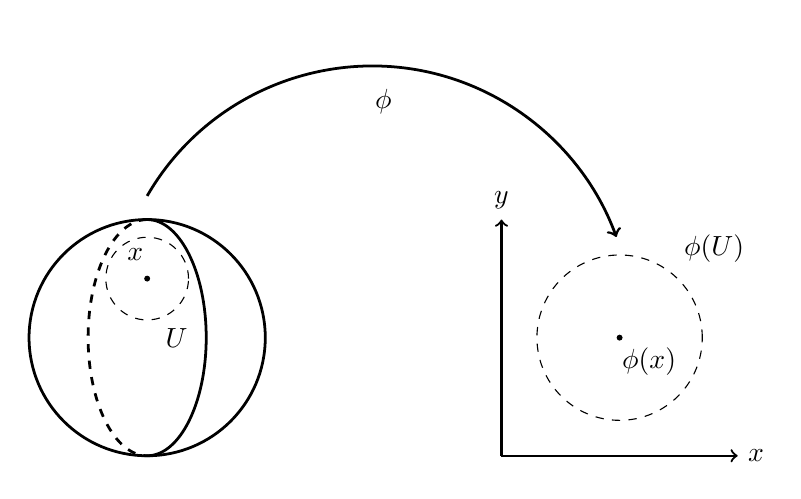
\begin{tikzpicture}[scale=1.5]
  \draw[line width=1] (-3,2) arc (90:-90:0.5 and 1);
  \draw[line width=1, dashed] (-3,2) arc (90:270:0.5 and 1);
  \draw[line width=1](-3,1) circle (1);
  \draw[color=black,thick,->] (0,0) -- (2,0) node[anchor=west]{$x$};
  \draw[color=black,thick,->] (0,0) -- (0,2) node[anchor=south]{$y$};

  \filldraw[black] (1,1) circle (0.02);
  \draw[dashed] (1,1) circle (0.7);
  \draw node at (1.25,0.80) {$\phi(x)$};
  \draw node at (1.8,1.75) {$\phi(U)$};

  \filldraw[black] (-3,1.5) circle (0.02);
  \draw node at (-3.1,1.70) {$x$};
  \draw[dashed] (-3,1.5) circle (0.35);
  \draw node at (-2.75,1) {$U$};

  \draw[line width=1, ->] (-3,2.2) arc (150:20:2.2);
  \draw node at (-1,3) {$\phi$};
\end{tikzpicture}

  \caption{Ejemplo de un homeomorfismo de una variedad a $\R^{2}$.}
\end{figure}
\end{frame}

\begin{frame}
\frametitle{Ejemplo de Variedades Topológicas}
\begin{columns}[t]
\column{.5\textwidth}
\centering
  \begin{figure}
    \scalebox{.5}{\tdplotsetmaincoords{70}{135}
\begin{tikzpicture}[scale=3,line join=bevel,tdplot_main_coords]
{\draw[color=black,thick,->] (0,0,0) -- (1,0,0) node[anchor=north east]{$x$};}%
{\draw[color=black,thick,->] (0,0,0) -- (0,1,0) node[anchor=north west]{$y$};}%
{\draw[color=black,thick,->] (0,0,0) -- (0,0,1) node[anchor=south]{$z$};}%
\end{tikzpicture}
}\\
    \caption{Los Espacios Euclidianos, $\R^n$.}
  \end{figure}
  \begin{figure}
    \scalebox{.5}{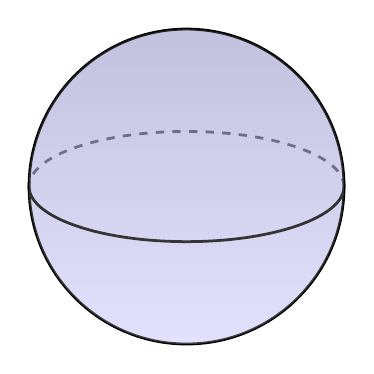
\begin{tikzpicture}[scale=2]
  \draw[line width=1, dashed] (1,0) arc (0:180:1 and 0.35);
  \draw[fill=blue!30!white!,opacity=0.5] (0,0) circle (1);
  \draw[line width=1] (1,0) arc (0:180:1 and -0.35);
  \draw[line width=1](0,0) circle (1);
  \shade[opacity=0.25] (0,0) circle (1);
\end{tikzpicture}

}\\
  \caption{La $n-$esferas, $\S^n$.}
  \end{figure}
\column{.5\textwidth}
\centering
  \begin{figure}
    \scalebox{.5}{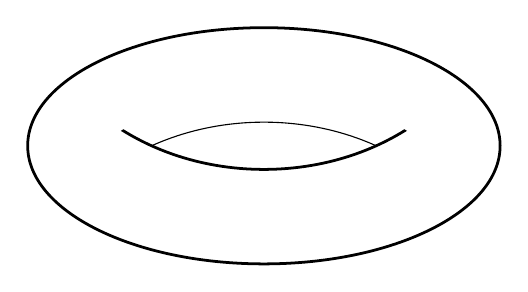
\begin{tikzpicture}
  \useasboundingbox (-3,-1.5) rectangle (3,1.5);
  \draw[line width=1] (0,0) ellipse (3 and 1.5);
  \begin{scope}
    \clip (0,-1.8) ellipse (3 and 2.5);
    \draw[line width=1] (0,2.2) ellipse (3 and 2.5);
  \end{scope}
  \begin{scope}
    \clip (0,2.2) ellipse (3 and 2.5);
    \draw (0,-2.2) ellipse (3 and 2.5);
  \end{scope}
\end{tikzpicture}
}\\
    \caption{El $n-$Toro, $\mathbb{T}^n$.}
  \end{figure}
  \begin{figure}
    \centering
    \scalebox{.5}{\begin{tikzpicture}[scale=4.5]
{\draw[color=black,thick,->] (0,0) -- (1,0) node[anchor=west]{$x$};}%
{\draw[color=black,thick,->] (0,0) -- (0,1) node[anchor=south]{$y$};}%
\draw[dashed] (0.5,0.5) circle (0.25);
\filldraw[black] (0.5,0.5) circle (0.02);
\end{tikzpicture}
}\\
    \caption{Los subconjuntos abiertos\\ de las variedades.}
  \end{figure}
\end{columns}
\end{frame}

\begin{frame}
\frametitle{Ejemplo: El Espacio Proyectivo}
\centering
\begin{figure}
  \scalebox{0.75}{\begin{tikzpicture}[scale=1.75]
\draw[color=black] (-2,0) -- (2,0);
\draw[color=black] (0,-2) -- (0,2);
\draw[thick] (0,0) circle (1);
\draw[thick] (-1.5, -1.5) -- (1.5,1.5); 
\filldraw[red] (0.71,0.71) circle (0.04);
\filldraw[blue] (-0.71,-0.71) circle (0.04);
\end{tikzpicture}
}
  \caption{Representación del Espacio Proyectivo $\mathbb{RP}^{2}$.}
.\end{figure}
\end{frame}

\begin{frame}
\frametitle{Cartas}
\begin{definition}[Carta]
  Una \textbf{carta} en $M$ es un par ordenado $(U,\phi)$ donde $U$ es un subconjunto abierto de $M$ y $\phi$ es un homeomorfismo de $U$ a $\R^n$.
\end{definition}\pause

\begin{definition}[Cartas Suavemente Compatibles]
  Si $(U,\phi)$ y $(V,\psi)$ son dos cartas en $M$ tales que $U \cap V \neq \varnothing$, llamaremos \textbf{mapa de transición} a la composición de funciones:
  \[ \psi \circ \phi^{-1}: \phi(U \cap V) \to \psi(U \cap V) \]
  
  Y además diremos que las cartas $(U,\phi)$ y $(V,\psi)$ son \textbf{suavemente compatibles} si $U \cap V = \varnothing$ o si el mapa de transición $\psi \circ \phi^{-1}$ es un difeomorfismo.
\end{definition}
\end{frame}

\begin{frame}
  \centering
  \begin{figure}
    \begin{tikzpicture}[scale=1]
	\coordinate (a) at (0,0);
	\path[draw,use Hobby shortcut,closed=true,thick]
	(0,2.5) .. (2,2.5) .. (1,4.5) .. (.3,4.5) .. (-1,4) .. (-2,2.5);

	\begin{scope}
		\clip (0.25,3.5) circle (0.5);
		\fill[blue!30!white,opacity=0.5] (-0.25,3.25) circle (0.5);
	\end{scope}
	\draw[dashed] (0.25,3.5) circle (0.5);
	\draw[dashed] (-0.25,3.25) circle (0.5);
	\draw node at (0.8,4) {$V$};
	\draw node at (-0.9,2.75) {$U$};

	\draw [thick, <->] (-5,0) -- (-1,0);
	\draw [thick, <->] (-3,-2) -- (-3,2);
	\draw [thick, <->] (1,0) -- (5,0);
	\draw [thick, <->] (3,-2) -- (3,2);

	\begin{scope}
		\clip (-3,0.5) ellipse  (0.8 and 1);
    \fill[color=blue!30!white,opacity=0.5] (-2.5,0) ellipse  (1.2 and 0.8);
	\end{scope}
	\draw [dashed,thick] (-3,0.5) ellipse  (0.8 and 1);
	% \draw [dashed,thick] (-2.5,0) ellipse  (1.2 and 0.8);

	\begin{scope}
		\clip (3,0.5) ellipse  (0.8 and 1);
		\fill[color=blue!30!white,opacity=0.5](3.5,0) ellipse  (1.2 and 0.8);
	\end{scope}
	% \draw [dashed,thick] (3,0.5) ellipse  (0.8 and 1);
	\draw [dashed,thick] (3.5,0) ellipse  (1.2 and 0.8);

	\draw[line width=1, ->] (1,3.75) arc (90:-5:2.5);
	\draw[line width=1, ->] (-1,3.25) arc (-90:0:-1.5);
	\draw[line width=1, ->] (-1.75,0.5) -- (2,0.5);

	\draw node at (-2.5,2.75) {$\phi$};
	\draw node at (3.25,3) {$\psi$};
	\draw node at (-4.25,1.25) {$\phi(U)$};
	\draw node at (4.5,1) {$\psi(V)$};
	\draw node at (0.25,1) {$\psi \circ \phi^{-1}$};


\end{tikzpicture}
  
    \caption{Mapa de Transición}
  \end{figure}
\end{frame}

\begin{frame}
  \frametitle{Atlas y la Estructura Suave}
  \begin{definition}[Atlas, Atlas Suave y Atlas Maximal]
    \begin{itemize}
      \item Una colección de cartas $(U,\phi)_{\alpha}$ es un \textbf{atlas} $\mathcal{A}$, en $M$ si dichas cartas forman una cubierta para $M$.
      \item Diremos que el atlas $\mathcal{A}$ es \textbf{suave} si cualesquiera dos cartas son suavemente compatibles, a las cartas de un atlas suaves les llamaremos \textit{cartas suaves}.
      \item Un atlas suave es llamado \textbf{maximal} si no está propiamente contenido en ningún atlas más grande.
    \end{itemize}
  \end{definition}\pause

  \begin{definition}[Variedad Suave]
    Si $M$ es una variedad topológica y $\mathcal{A}$ es un atlas maximal en $M$, diremos que el par $(M,\mathcal{A})$ es una \textbf{variedad suave}, a dicho atlas maximal le llamaremos la \textbf{estructura suave} en $M$.
  \end{definition}
\end{frame}


\begin{frame}
\frametitle{Ejemplo de Variedades Suaves}
\begin{columns}[t]
\column{.5\textwidth}
\centering
  \begin{figure}
    \scalebox{.5}{\tdplotsetmaincoords{70}{135}
\begin{tikzpicture}[scale=3,line join=bevel,tdplot_main_coords]
{\draw[color=black,thick,->] (0,0,0) -- (1,0,0) node[anchor=north east]{$x$};}%
{\draw[color=black,thick,->] (0,0,0) -- (0,1,0) node[anchor=north west]{$y$};}%
{\draw[color=black,thick,->] (0,0,0) -- (0,0,1) node[anchor=south]{$z$};}%
\end{tikzpicture}
}\\
    \caption{Los Espacios Euclidianos, $\R^n$.}
  \end{figure}
  \begin{figure}
    \scalebox{.5}{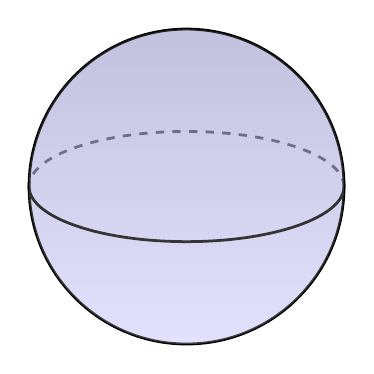
\begin{tikzpicture}[scale=2]
  \draw[line width=1, dashed] (1,0) arc (0:180:1 and 0.35);
  \draw[fill=blue!30!white!,opacity=0.5] (0,0) circle (1);
  \draw[line width=1] (1,0) arc (0:180:1 and -0.35);
  \draw[line width=1](0,0) circle (1);
  \shade[opacity=0.25] (0,0) circle (1);
\end{tikzpicture}

}\\
  \caption{La $n-$esferas, $\S^n$.}
  \end{figure}
\column{.5\textwidth}
\centering
  \begin{figure}
    \scalebox{.5}{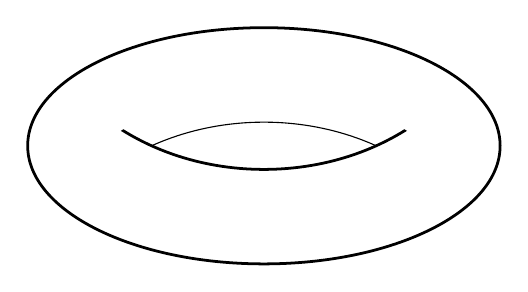
\begin{tikzpicture}
  \useasboundingbox (-3,-1.5) rectangle (3,1.5);
  \draw[line width=1] (0,0) ellipse (3 and 1.5);
  \begin{scope}
    \clip (0,-1.8) ellipse (3 and 2.5);
    \draw[line width=1] (0,2.2) ellipse (3 and 2.5);
  \end{scope}
  \begin{scope}
    \clip (0,2.2) ellipse (3 and 2.5);
    \draw (0,-2.2) ellipse (3 and 2.5);
  \end{scope}
\end{tikzpicture}
}\\
    \caption{El $n-$Toro, $\mathbb{T}^n$.}
  \end{figure}
  \begin{figure}
    \centering
    \scalebox{.5}{\begin{tikzpicture}[scale=4.5]
{\draw[color=black,thick,->] (0,0) -- (1,0) node[anchor=west]{$x$};}%
{\draw[color=black,thick,->] (0,0) -- (0,1) node[anchor=south]{$y$};}%
\draw[dashed] (0.5,0.5) circle (0.25);
\filldraw[black] (0.5,0.5) circle (0.02);
\end{tikzpicture}
}\\
    \caption{Subconjuntos abiertos\\ de variedades suaves.}
  \end{figure}
\end{columns}
\end{frame}
